\section{Realizarea lucrarii de laborator}

\subsection{Tasks and Points}
\begin{itemize}
	\item Basic Level (nota 5 || 6):
	
	\begin{itemize}
		\item Realizeaza un simplu GUI calculator care suporta functiile de baza: +, -, /, *.
	\end{itemize}
	
	\item Normal Level (nota 7 || 8):
	
	\begin{itemize}
		\item Realizeaza un simplu GUI calculator care suporta urmatoare functii: +, -, /, *, putere, radical, InversareSemn(+/-).
	\end{itemize}
	\item Advanced Level (nota 9 || 10):
	
	\begin{itemize}
		\item Realizeaza un simplu GUI calculator care suporta urmatoare functii: +, -, /, *, putere, radical, InversareSemn(+/-), operatii cu numere zecimale.
	\end{itemize}
	\begin{itemize}
		\item Divizare proiectului in doua module - Interfata grafica(Modul GUI) si Modulul de baza(Core Module).
	\end{itemize}
\end{itemize}
\subsection{Analiza lucrarii de laborator}

 
 

Am realizat Calculatorul folosind IDE-ul in limbajul \textsc{\large C\#} folosind un proiect de tip Xaml Calculatorul final:\\
\begin{center}
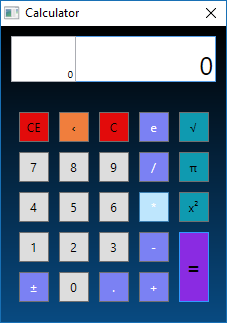
\includegraphics[scale=1]{images/1}
\end{center}
Interfata grafica a calculatorului am utlizat diferite componente din Visual Studio si le-am amplasat in fereastra ,la calculator am utilizat componente ca:button,TextBox si Label.
Butoanele predestinate pentru operatii,TextBox pentru afisarea rezultatelor si cifrele care sunt introduse utilizind mouse-ul si tastatura, si Label-ul pentru afisarea cifrelor si operatiilor curente.Cind selectam un buton in modul grafic putem modifica : caption,color,font,style,name,etc.La realizarea functionalul pentru butoane am utilizat functii globale care extrag din cimpul text a butonului valoarea pentru a fi utilizata la calcule.Utilizind functii universale am optimizat codul,in rezultat nu a fost necesar sa implementez functii pentru fiecare button.

\section{Imagini}
Imaginea finala a calculatorului creat.
\begin{center}
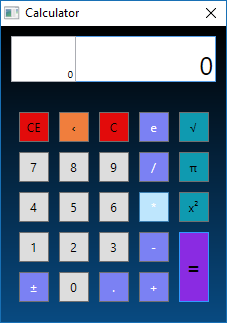
\includegraphics[scale=1]{images/1}

\end{center}
\begin{center}
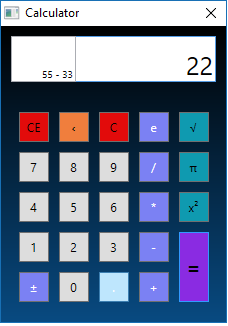
\includegraphics[scale=1]{images/2}

\end{center}
\clearpage